\section{Forward Model and Observable Mapping}
\label{sec:model}

The forward model used in this paper is a steady, one-dimensional description of a starburst-driven multiphase wind.
It follows the classical picture in which supernovae and stellar winds thermalize inside a compact launch region and drive a hot, volume-filling outflow \citep{Chevalier85}.
The model then embeds cool clouds in this hot wind and evolves the two phases together as they exchange mass, momentum, and energy through turbulent, radiatively cooling interfaces \citep{Fielding22}.
The calculation is intentionally reduced: it does not attempt to resolve the cloud-wind interface directly, nor does it model the full three-dimensional geometry of a real outflow.
Instead, it asks whether a physically controlled radial model can map a small set of wind and cloud parameters into the cool-gas velocity and column-density distributions measured in absorption.

The main extension relative to the single-cloud implementation used in earlier applications is that the cool phase is represented by a mass spectrum.
The injected cool material is divided into logarithmically spaced cloud-mass bins, and each bin evolves as a separate cloud species with its own mass, velocity, metallicity, size, cooling parameter, and contribution to the final column-density profile.
This matters because small clouds are numerous and couple efficiently to the hot phase, while larger clouds can survive longer and carry substantial cold mass to larger radii.
The observable profile is therefore not the trajectory of one representative cloud, but the sum of many cloud species that respond differently to the same hot wind.
This section defines that forward map.
The statistical machinery used to fit or validate the model is introduced only after the physical model has been specified.

\subsection{Model Geometry and Hot-Wind Launch}
\label{subsec:model_launch}

We consider a radial wind subtending a solid angle $\Omega_{\rm wind}$.
The model is initialized at a characteristic launch radius $r_\star$, which should be interpreted as the radius at which the hot wind has passed through the sonic point and begins to interact with the cool cloud population followed in the calculation.
For a galaxy with star formation rate $\dot{M}_\star$, the hot phase is specified by two dimensionless loading factors.
The hot mass loading is
\begin{equation}
\dot{M}_{\rm hot} = \eta_M \dot{M}_\star ,
\end{equation}
and the hot energy injection rate is
\begin{equation}
\dot{E}_{\rm hot}
=
\eta_E
\frac{E_{\rm SN}}{m_\star}
\dot{M}_\star .
\end{equation}
Here $E_{\rm SN}$ is the mechanical energy per supernova and $m_\star$ is the stellar mass formed per supernova.
The ratio $\dot{E}_{\rm hot}/\dot{M}_{\rm hot}$ sets the specific energy of the hot wind, while $\eta_M$ and $\eta_E$ separately control the hot density, pressure, and cooling rate.

The launch state is set by imposing a Mach number slightly offset from unity,
\begin{equation}
{\cal M}_0 = 1 + \epsilon_{\rm sonic}.
\end{equation}
This small offset regularizes the transonic initial condition while keeping the solution tied to the sonic point.
In the current implementation the hot velocity at $r_\star$ is
\begin{equation}
v_\star =
\left(\frac{\dot{E}_{\rm hot}}{\dot{M}_{\rm hot}}\right)^{1/2}
\left[
\frac{1}{(\gamma-1){\cal M}_0}
+ \frac{1}{2}
\right]^{-1/2},
\end{equation}
with density fixed by mass-flux conservation,
\begin{equation}
\rho_\star =
\frac{\dot{M}_{\rm hot}}
{\Omega_{\rm wind} r_\star^2 v_\star},
\end{equation}
and pressure fixed by the Mach-number definition,
\begin{equation}
P_\star =
\frac{\rho_\star v_\star^2}{\gamma {\cal M}_0^2}.
\end{equation}
These equations are the implemented launch convention used by the calculations in this paper.
The same mass and energy injection rates also define source terms inside the launch region, normalized by the volume $4\pi r_\star^3/3$.
The flux normalization outside the launch region retains the explicit wind solid angle $\Omega_{\rm wind}$.

Gravity is represented by an isothermal potential,
\begin{equation}
\Phi(r) = v_{\rm circ}^2 \ln r ,
\end{equation}
where $v_{\rm circ}$ is the circular velocity of the galaxy.
Thus the fixed galaxy inputs that determine the hot-wind background are $\dot{M}_\star$, $r_\star$, $v_{\rm circ}$, and $\Omega_{\rm wind}$.
Increasing $\eta_E/\eta_M$ raises the specific energy and therefore the characteristic launch speed.
Increasing $\eta_M$ at fixed $\eta_E/\eta_M$ raises the hot density and makes radiative cooling and cloud coupling more important.
Changing $r_\star$ shifts the density scale through the area of the launch surface, while $v_{\rm circ}$ controls how strongly gravity decelerates the outflow.

\begin{figure*}[!htbp]
\centering
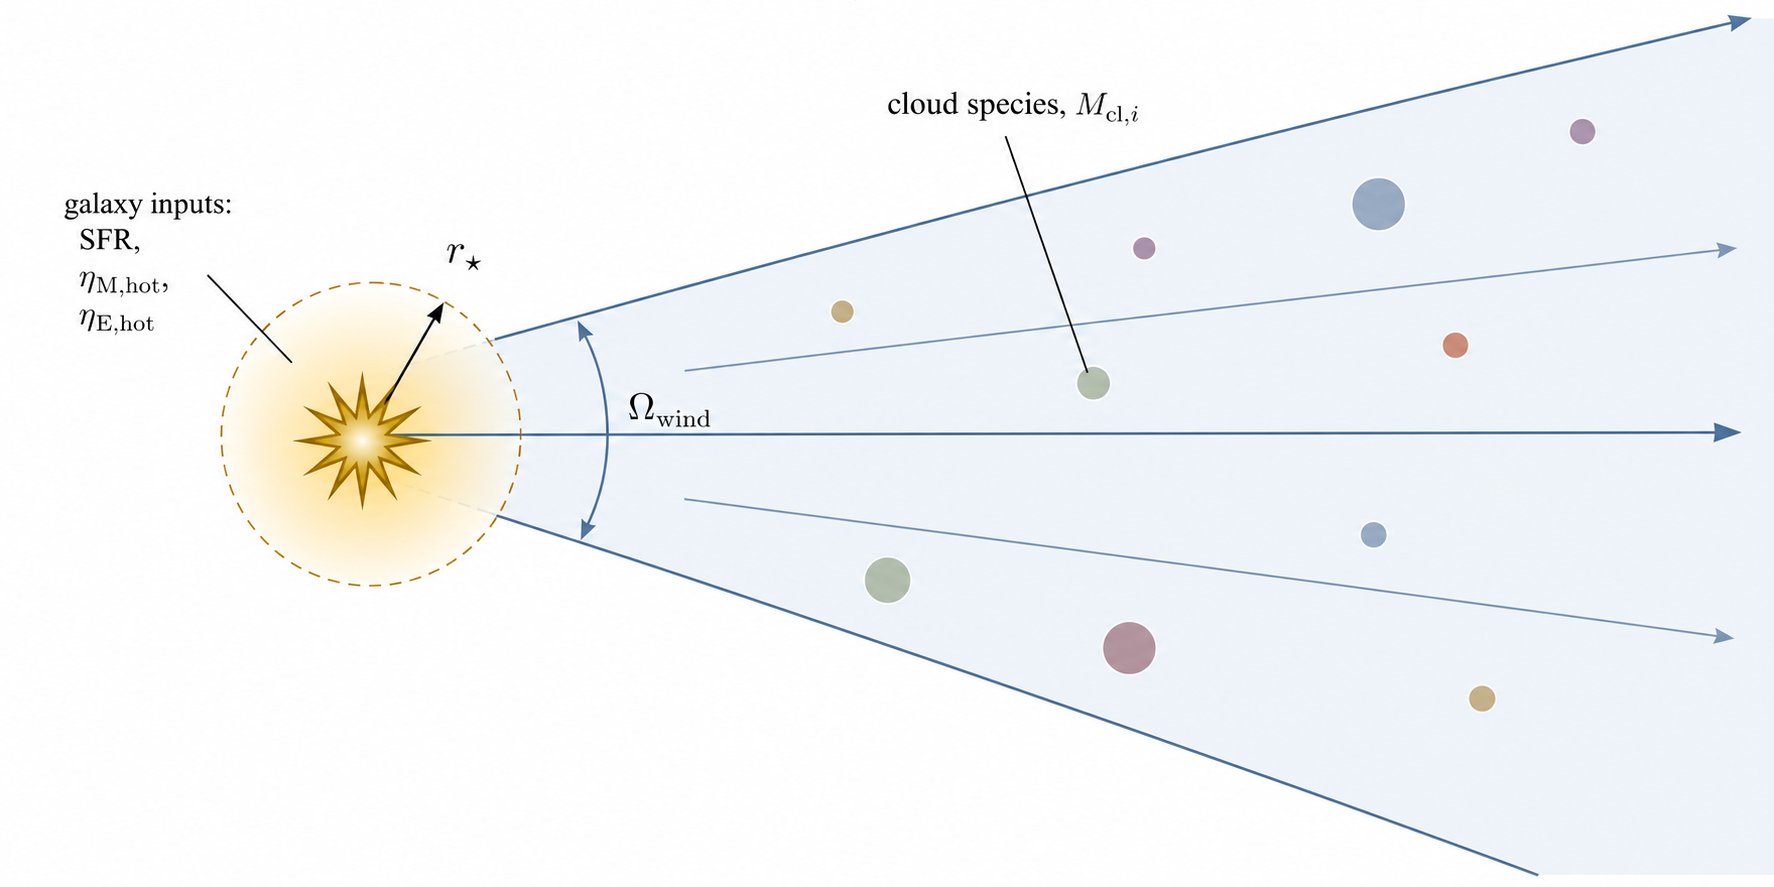
\includegraphics[width=0.92\textwidth]{figures/forward_model_launch_geometry.png}
\caption{
Conceptual geometry of the forward model launch region.
The hot wind is initialized at $r_\star$ after passing through the sonic point and then evolves radially through a straight biconical solid angle $\Omega_{\rm wind}$.
The launch region is set by the star formation rate and the hot mass and energy loading factors, while the colored circles indicate that the cool phase is represented by multiple cloud species with different initial masses.
This schematic is a guide to the implemented geometry and source terms, not a fit to any individual galaxy.
The numerical calculation is carried out in CGS units internally, while the user-facing quantities that set this launch problem include $\dot{M}_\star$, $\eta_{M,{\rm hot}}$, $\eta_{E,{\rm hot}}$, $r_\star$, and $\Omega_{\rm wind}$.
}
\label{fig:model_launch_geometry}
\end{figure*}

\subsection{Cold Cloud Mass Spectrum}
\label{subsec:model_cloud_spectrum}

The new ingredient in this paper is the explicit cloud mass spectrum.
Instead of choosing one representative cloud mass, we divide the injected cool phase into $N_{\rm cl}$ logarithmically spaced representative masses,
\begin{equation}
M_{{\rm cl},i}
=
10^{\log_{10}M_{\rm cl,min}+(i-1)\Delta\log_{10}M_{\rm cl}},
\end{equation}
where
\begin{equation}
\Delta\log_{10}M_{\rm cl}
=
\frac{\log_{10}M_{\rm cl,max}-\log_{10}M_{\rm cl,min}}{N_{\rm cl}-1}.
\end{equation}
These masses should be interpreted as species labels for a discretized cloud population, not as a claim that real clouds form at only these masses.
The continuous number injection spectrum is taken to be a power law,
\begin{equation}
\frac{d\dot{N}_{\rm cl}}{dM_{\rm cl}}
\propto
M_{\rm cl}^{-\alpha_{\rm cl}},
\end{equation}
or, equivalently,
\begin{equation}
\frac{d\dot{N}_{\rm cl}}{d\log_{10} M_{\rm cl}}
\propto
M_{\rm cl}^{1-\alpha_{\rm cl}}.
\end{equation}
The discrete relative number weight of species $i$ is therefore
\begin{equation}
w_{N,i}
=
M_{{\rm cl},i}^{1-\alpha_{\rm cl}}\Delta\log_{10} M_{\rm cl},
\end{equation}
up to an arbitrary normalization that cancels below.
The corresponding relative cold mass weight is
\begin{equation}
w_{M,i}
=
M_{{\rm cl},i}w_{N,i}.
\end{equation}

The total cold mass injection rate is set by a third loading factor,
\begin{equation}
\dot{M}_{\rm cold,tot}
=
\eta_{M,{\rm cold}}\dot{M}_\star .
\end{equation}
We assign this total flux to the discrete species according to the mass fraction
\begin{equation}
f_{M,i}
=
\frac{w_{M,i}}{\sum_j w_{M,j}},
\end{equation}
so that
\begin{equation}
\eta_{M,{\rm cold},i}
=
\eta_{M,{\rm cold}} f_{M,i},
\end{equation}
\begin{equation}
\dot{M}_{{\rm cold},i}
=
\eta_{M,{\rm cold},i}\dot{M}_\star ,
\end{equation}
\begin{equation}
\dot{N}_{{\rm cl},i}
=
\frac{\dot{M}_{{\rm cold},i}}{M_{{\rm cl},i}}.
\end{equation}
This construction separates the total amount of cold material, controlled by $\eta_{M,{\rm cold}}$, from how that material is divided among many cloud sizes, controlled by $\alpha_{\rm cl}$ and the cloud-mass bounds.
It also makes clear why $\alpha_{\rm cl}=2$ is a useful fiducial case.
For this slope, $w_{M,i}\propto M_{{\rm cl},i}^{2-\alpha_{\rm cl}}$ is approximately independent of mass, so each logarithmic mass interval receives a comparable share of the injected cold mass.
The number flux is very different: at fixed mass per logarithmic interval, the lowest-mass bins contain many more clouds.
This separation between mass weighting and number weighting is the central reason that a mass spectrum cannot usually be replaced by one effective cloud.
Figure~\ref{fig:cloud_mass_spectrum_initialization} shows this initialization for the fiducial spectrum used in the baseline inference tests.

\begin{figure*}[!htbp]
\centering
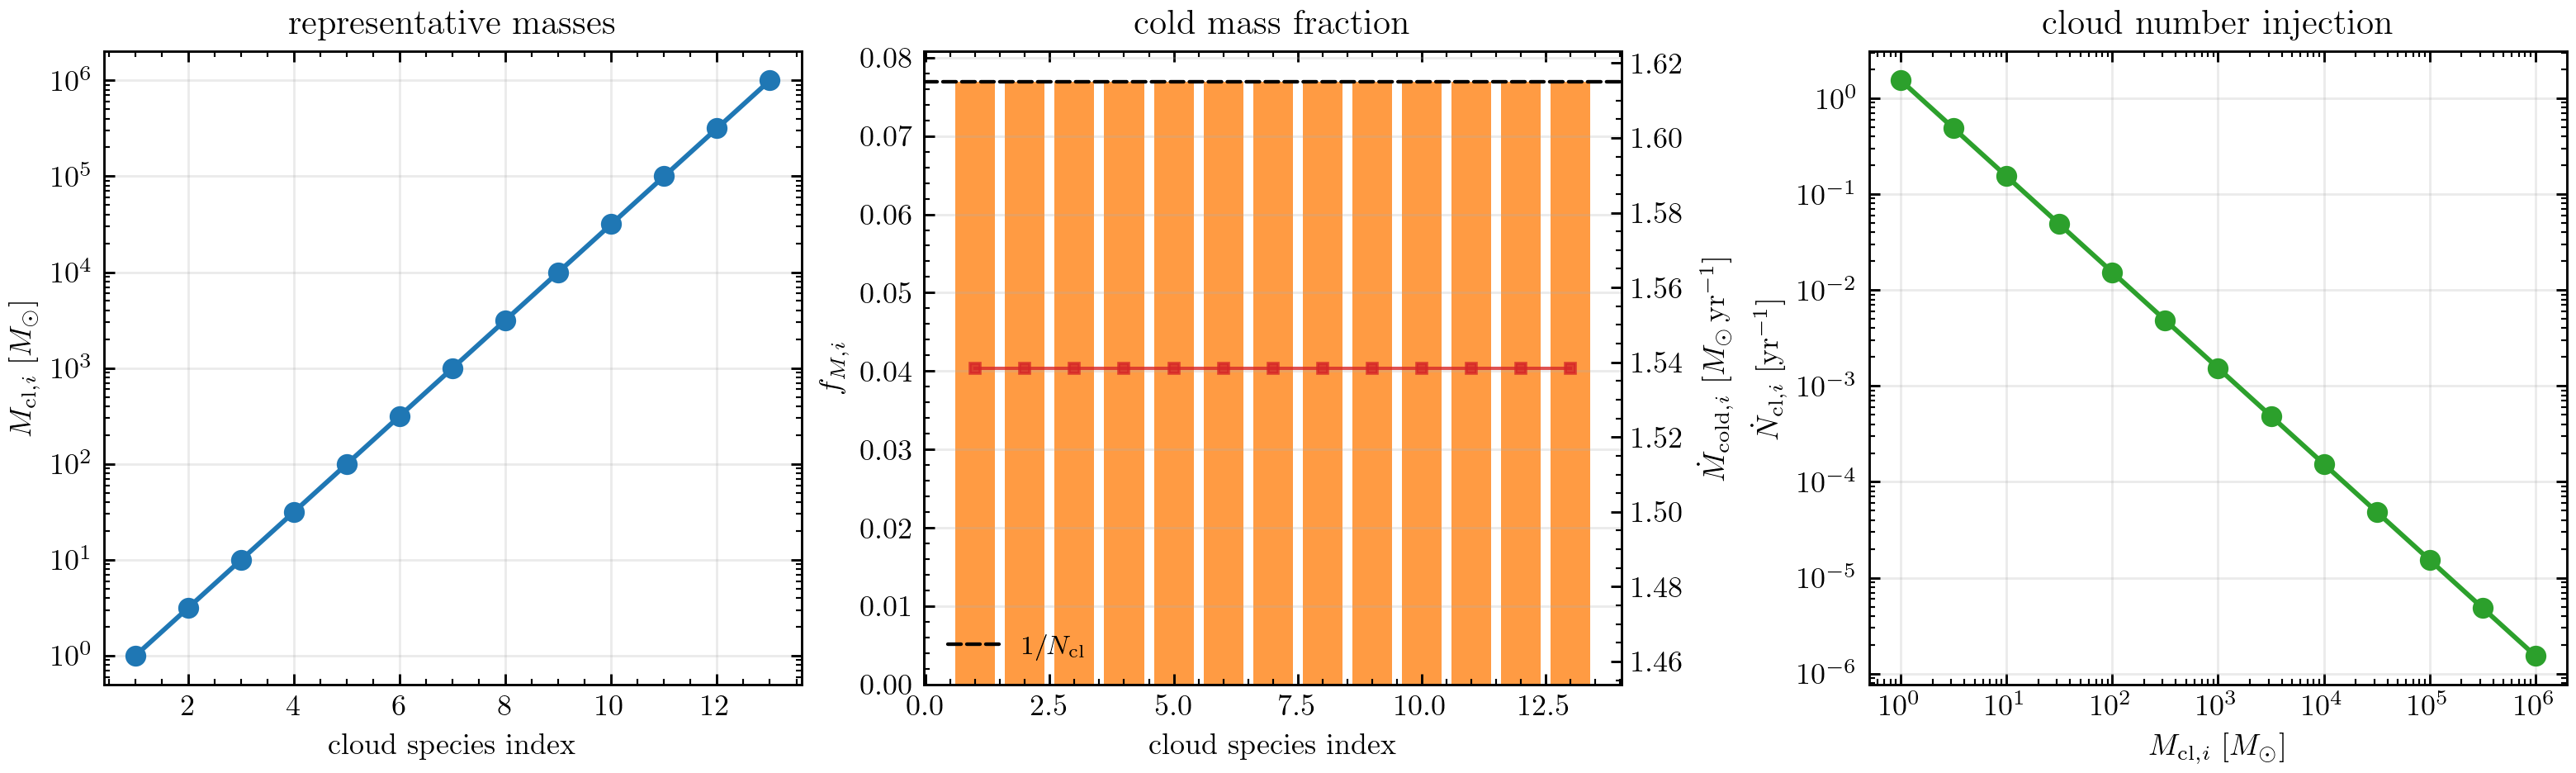
\includegraphics[width=\textwidth]{figures/cloud_mass_spectrum_initialization.png}
\caption{
Fiducial initialization of the cold cloud mass spectrum.
The representative masses span $M_{\rm cl,min}=1\,M_\odot$ to $M_{\rm cl,max}=10^6\,M_\odot$ with $N_{\rm cl}=13$ logarithmically spaced species.
For the default slope $\alpha_{\rm cl}=2$ and total cold mass loading $\eta_{M,{\rm cold}}=1$, the cold mass fraction is nearly flat across logarithmic mass bins, while the number injection rate falls approximately as $M_{\rm cl}^{-1}$.
Thus small clouds dominate the number budget even though they do not dominate the injected cold mass.
The plotted mass flux assumes $\dot{M}_\star=20\,M_\odot\,{\rm yr}^{-1}$.
}
\label{fig:cloud_mass_spectrum_initialization}
\end{figure*}

\subsection{Cloud Injection and Number Density}
\label{subsec:model_cloud_injection}

The quantities above define the asymptotic cloud number flux associated with each species.
In the implemented model, that flux is introduced over a finite radial interval rather than being switched on discontinuously at the launch radius.
Each cloud species has a radial number flux
\begin{equation}
\dot{N}_i(r)
=
\dot{N}_{i,0} I(r),
\end{equation}
where the injection profile is
\begin{equation}
I(r) =
\left\{
\begin{array}{ll}
\left(r/r_{\rm inj}\right)^{p_{\rm inj}}, & r < r_{\rm inj},\\
1, & r \ge r_{\rm inj}.
\end{array}
\right.
\end{equation}
The injection radius is tied to the hot-wind launch radius by
\begin{equation}
r_{\rm inj}
=
f_{\rm inj}r_\star .
\end{equation}
The current default values are $f_{\rm inj}=1.33$ and $p_{\rm inj}=6$.
This choice makes the cloud source term rise steeply just outside the launch region and reach its full value by $r_{\rm inj}$.
Flux conservation then gives the local number density of species $i$,
\begin{equation}
n_{{\rm cl},i}
=
\frac{\dot{N}_i(r)}
{\Omega_{\rm wind} r^2 v_{{\rm cl},i}}.
\end{equation}
The hot phase couples to the cold phase through sums over species of the form $n_{{\rm cl},i}\dot{M}_i$, $n_{{\rm cl},i}\dot{p}_i$, and $n_{{\rm cl},i}\dot{e}_i$.
This is where the mass spectrum matters dynamically.
The geometric factor $\Omega_{\rm wind}r^2$ dilutes all species in the same way, while the velocity factor accounts for residence time along the radial flow.
At fixed $v_{{\rm cl},i}$, species with larger $\dot{N}_{i,0}$ have larger number densities and therefore contribute more individual cloud interfaces per unit volume.
For the fiducial $\alpha_{\rm cl}=2$ initialization, this means that low-mass clouds can dominate the cloud count even when the cold mass density is initially distributed nearly evenly over logarithmic mass.
The subsequent evolution can then break this simple initialization because different masses accelerate, grow, and disrupt at different rates.
Figure~\ref{fig:cloud_injection_number_density} isolates the initialization effect before those dynamical differences appear.

\begin{figure}[!htbp]
\centering
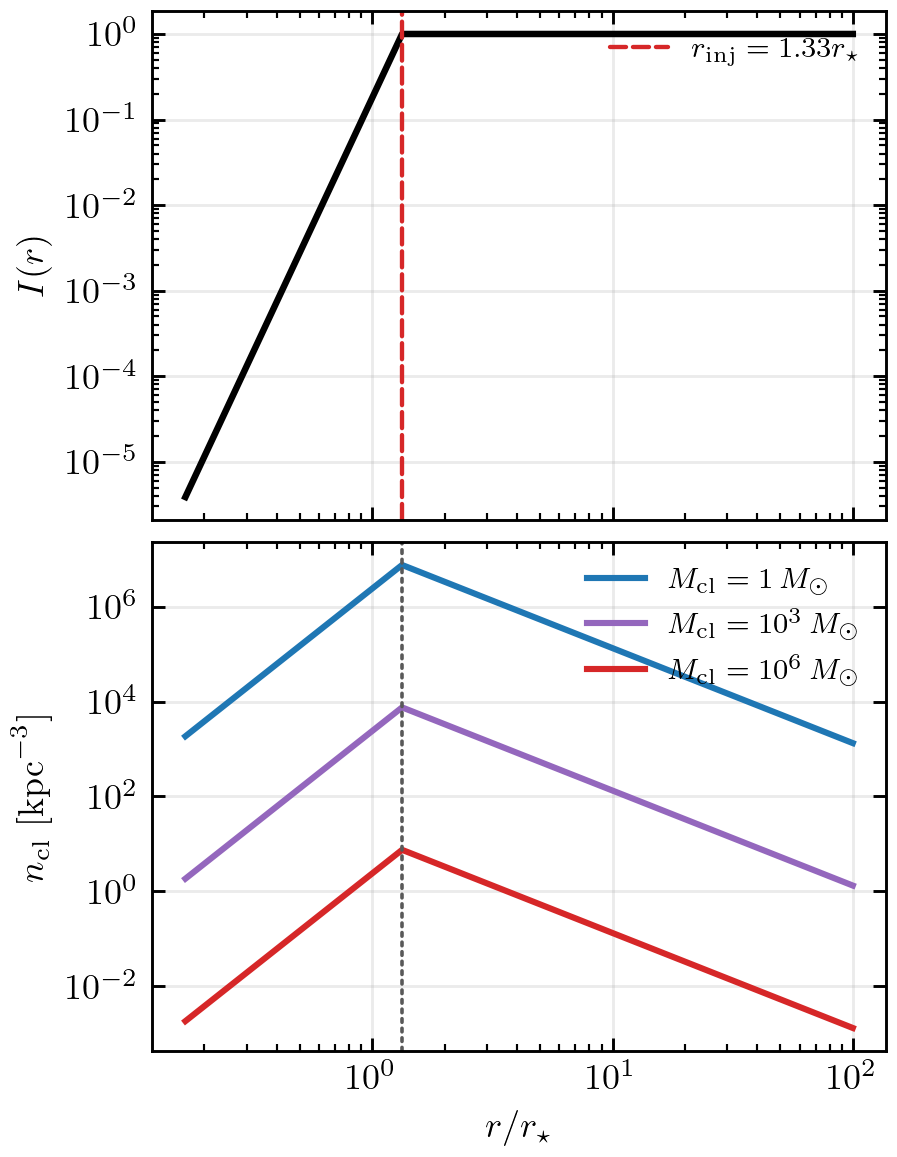
\includegraphics[width=\columnwidth]{figures/cloud_injection_number_density.png}
\caption{
Radial injection and initial number-density structure for the same fiducial cloud spectrum shown in Figure~\ref{fig:cloud_mass_spectrum_initialization}.
The top panel shows the implemented injection profile $I(r)$ with $r_{\rm inj}=1.33r_\star$ and $p_{\rm inj}=6$.
The bottom panel shows the corresponding cloud number density for three representative mass bins, assuming $r_\star=0.3\,{\rm kpc}$, $\Omega_{\rm wind}=4\pi$, and a common initial cloud velocity $v_{\rm cl,0}=100\,{\rm km}\,{\rm s}^{-1}$.
The number density is plotted in ${\rm kpc}^{-3}$ for readability.
The strong vertical separation between the curves is not a dynamical effect; it follows directly from distributing comparable cold mass over logarithmic bins while assigning much smaller masses to the low-mass species.
}
\label{fig:cloud_injection_number_density}
\end{figure}

\subsection{Pressure Equilibrium and Mixing-Layer Cooling}
\label{subsec:model_mixing_layer}

The cold clouds are assumed to remain in pressure equilibrium with the hot phase.
This is the closure that turns the hot-wind solution into cloud sizes, density contrasts, and cooling times.
For a fixed cloud temperature $T_{\rm cl}$,
\begin{equation}
\rho_{{\rm cl},i}
=
\frac{P\mu m_p}{k_B T_{\rm cl}},
\end{equation}
and
\begin{equation}
R_{{\rm cl},i}
=
\left(
\frac{3M_{{\rm cl},i}}
{4\pi \rho_{{\rm cl},i}}
\right)^{1/3}.
\end{equation}
The density contrast is
\begin{equation}
\chi_i =
\frac{\rho_{{\rm cl},i}}{\rho_{\rm hot}}.
\end{equation}
Because the cloud and hot phase are in pressure equilibrium, this density contrast is also approximately $T_{\rm hot}/T_{\rm cl}$.
The interface model is then controlled by the competition between turbulent mixing and radiative cooling.
The turbulent radiative mixing layer is evaluated at the geometric-mean temperature and metallicity,
\begin{equation}
T_{{\rm mix},i}
=
\left(T_{\rm hot}T_{\rm cl}\right)^{1/2},
\end{equation}
\begin{equation}
Z_{{\rm mix},i}
=
\left(Z_{\rm hot}Z_{{\rm cl},i}\right)^{1/2}.
\end{equation}
The relevant cooling time is
\begin{equation}
t_{{\rm cool},i}
=
t_{\rm cool}
\left(T_{{\rm mix},i},P/k_B,Z_{{\rm mix},i}/Z_\odot\right).
\end{equation}
Here the pressure argument is written as $P/k_B$ in units of ${\rm K}\,{\rm cm}^{-3}$, matching the cooling-table convention used in the code.
If the tabulated cooling function enters a net-heating regime, the implementation treats the interface cooling time as effectively long rather than allowing a negative cooling time to reverse the condensation prescription.

The turbulent velocity is modeled as
\begin{equation}
v_{{\rm turb},i}
=
f_{\rm turb}
\left|v_{\rm hot}-v_{{\rm cl},i}\right|
\chi_i^{a_{\rm turb}},
\end{equation}
which defines the cooling parameter
\begin{equation}
\xi_i
=
\frac{R_{{\rm cl},i}}
{v_{{\rm turb},i}t_{{\rm cool},i}}.
\end{equation}
The quantity $\xi_i$ compares the cloud radius to the distance a turbulent eddy travels in one mixed-layer cooling time.
It is therefore the most compact way to see which regime an interface occupies.
For $\xi_i \gtrsim 1$, mixed gas can cool before being advected away from the cloud surface, making condensation more effective.
For $\xi_i \lesssim 1$, the interface is more nearly mixing dominated and cloud destruction is favored.
The same hot wind can place different cloud masses in different regimes because $R_{{\rm cl},i}\propto M_i^{1/3}$ at fixed pressure.
Figure~\ref{fig:mixing_layer_cooling_parameter} shows this explicitly for the fiducial solved model used in the method figures.

\begin{figure}[!htbp]
\centering
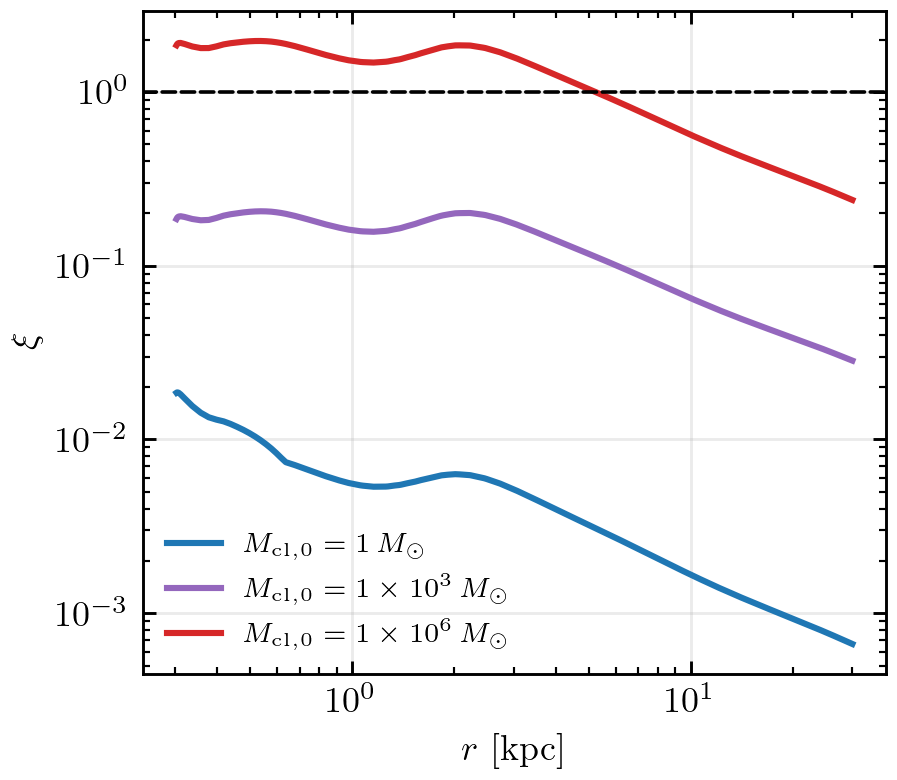
\includegraphics[width=\columnwidth]{figures/mixing_layer_cooling_parameter.png}
\caption{
Cooling parameter for three representative cloud species in the fiducial solved model.
The model uses $\dot{M}_\star=20\,M_\odot\,{\rm yr}^{-1}$, $v_{\rm circ}=150\,{\rm km}\,{\rm s}^{-1}$, $\eta_M=0.1$, $\eta_{M,{\rm cold}}=0.2$, $\eta_E=1$, and $r_\star=0.3\,{\rm kpc}$.
The dashed line marks $\xi=1$.
At fixed pressure, larger clouds have larger radii and therefore larger $\xi_i$, so they are closer to the radiatively efficient condensation regime than the low-mass species.
}
\label{fig:mixing_layer_cooling_parameter}
\end{figure}

\subsection{Cloud Mass Exchange}
\label{subsec:model_mass_exchange}

The model converts the cooling parameter into cloud growth and cloud loss rates.
For each active cloud species, the net cloud mass change is
\begin{equation}
\dot{M}_i =
\dot{M}_{{\rm grow},i}
+
\dot{M}_{{\rm loss},i}.
\end{equation}
The growth term is
\begin{equation}
\dot{M}_{{\rm grow},i}
=
C_M
\frac{3M_i v_{{\rm turb},i}}{R_i\chi_i}
A_i f_{\xi,i},
\end{equation}
where
\begin{equation}
A_i =
f_A \chi_i^{a_A},
\end{equation}
and
\begin{equation}
f_{\xi,i}
=
\left\{
\begin{array}{ll}
\xi_i^{1/2}, & \xi_i < 1,\\
\xi_i^{1/4}, & \xi_i \ge 1.
\end{array}
\right.
\end{equation}
The factor $A_i$ is an effective area enhancement for the turbulent interface, while $f_{\xi,i}$ encodes the change in condensation efficiency across the $\xi_i=1$ boundary.
The cloud mass-loss term is
\begin{equation}
\dot{M}_{{\rm loss},i}
=
-C_M
\frac{3M_i v_{{\rm turb,cold},i}}{R_i},
\end{equation}
with
\begin{equation}
v_{{\rm turb,cold},i}
=
v_{{\rm turb},i}\chi_i^{a_{\rm cold}}.
\end{equation}
These equations encode the central competition in the model.
Clouds grow when mixed gas cools rapidly enough to condense, and they lose mass when turbulent motions entrain cold gas into the hot flow faster than cooling can return it.
Clouds are removed from the active exchange terms once their mass falls below the implemented minimum cloud mass threshold.
This threshold prevents a numerically destroyed species from continuing to exert a spurious force through an arbitrarily small radius.

The important point for the mass-spectrum model is that the exchange rates do not scale linearly with cloud mass.
At fixed pressure, $R_i\propto M_i^{1/3}$, so the ratio $M_i/R_i$ scales as $M_i^{2/3}$, while the cooling parameter also grows as $M_i^{1/3}$.
Large clouds therefore have larger cooling parameters and longer survival times, but they are also less numerous at fixed total cold mass.
Small clouds present many interfaces to the hot wind and can couple strongly near the launch region, but they are more easily destroyed.
This is the physical reason that the multi-species model produces a distribution of cloud histories rather than a rescaled version of one trajectory.
Figure~\ref{fig:cloud_species_mass_velocity_evolution} shows the resulting divergence in mass survival and acceleration for representative species.

\begin{figure*}[!htbp]
\centering
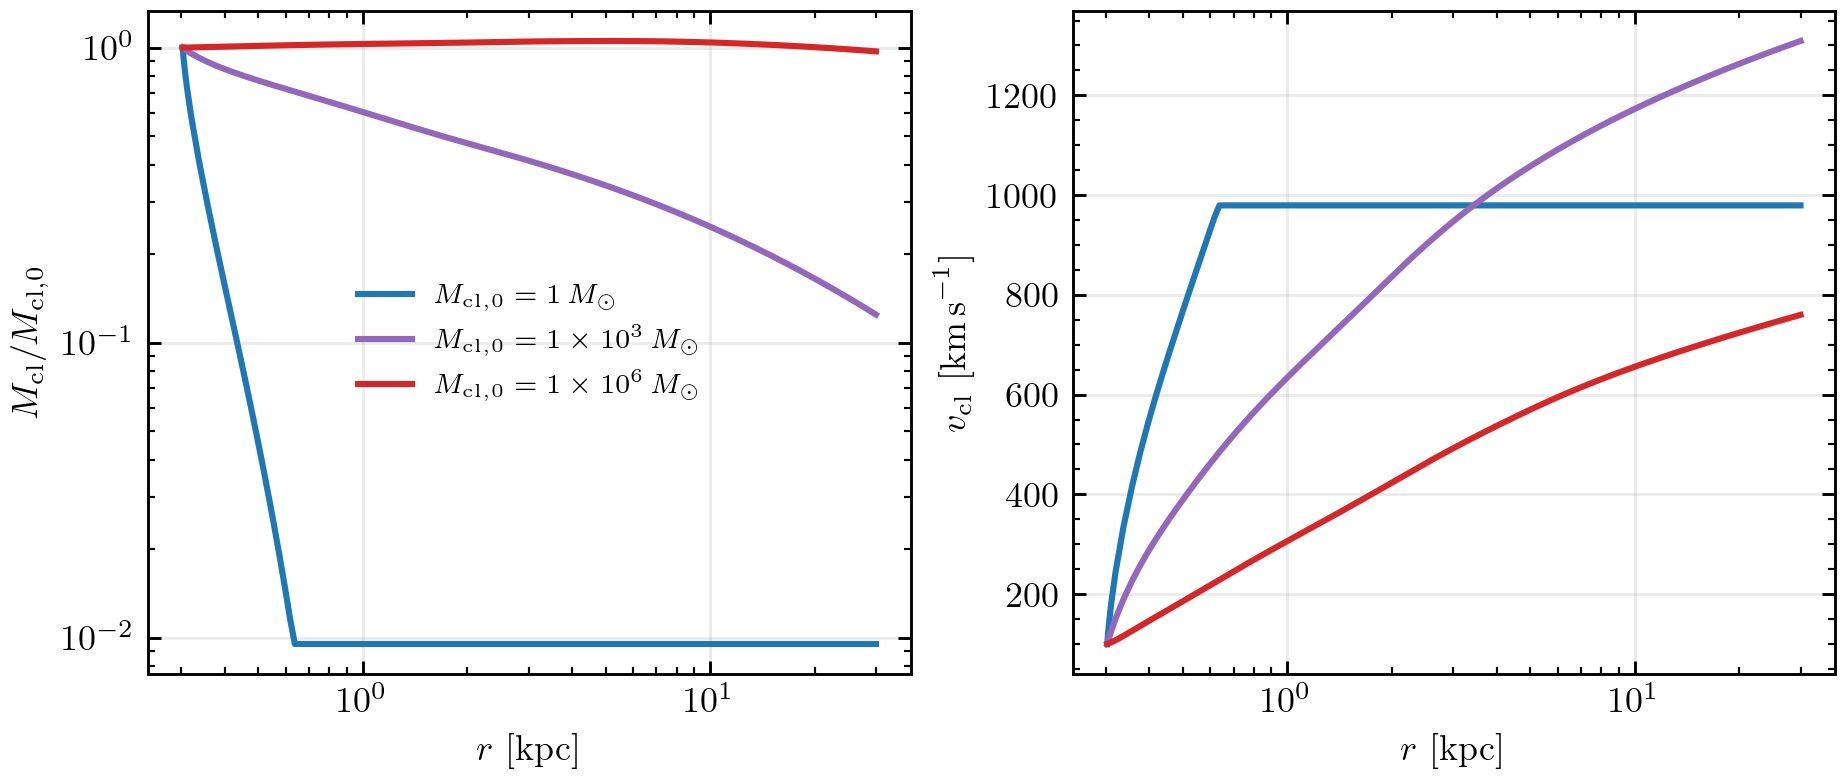
\includegraphics[width=0.78\textwidth]{figures/cloud_species_mass_velocity_evolution.png}
\caption{
Mass survival and acceleration of representative cloud species in the fiducial solved model.
The low-mass species has the smallest cooling parameter and is rapidly depleted, while the high-mass species survives to larger radius and accelerates more gradually.
The intermediate species illustrates that the transition between destruction and survival is continuous across the cloud mass spectrum.
These trajectories use the same fiducial parameters as Figure~\ref{fig:mixing_layer_cooling_parameter}; only three species are shown for clarity, but all thirteen species are included in the coupled wind calculation.
}
\label{fig:cloud_species_mass_velocity_evolution}
\end{figure*}

\subsection{Momentum and Energy Exchange}
\label{subsec:model_momentum_energy}

The mass exchange terms also carry momentum and energy.
The code treats two momentum channels separately: ram pressure on the cloud surface and the momentum advected by mass that changes phase.
The ram pressure force on species $i$ is
\begin{equation}
\dot{p}_{{\rm ram},i}
=
\frac{1}{2}C_D \rho_{\rm hot}
\pi R_i^2
v_{{\rm rel},i}\left|v_{{\rm rel},i}\right|,
\end{equation}
where $v_{{\rm rel},i}=v_{\rm hot}-v_i$.
With this convention, $\dot{p}_{{\rm ram},i}>0$ when the hot wind is faster than the cloud and the ram force accelerates the cloud outward.
The momentum carried by mass exchange is
\begin{equation}
\dot{p}_{{\rm trans},i}
=
v_{\rm hot}\dot{M}_{{\rm grow},i}
+
v_i\dot{M}_{{\rm loss},i}.
\end{equation}
The first term removes hot-wind momentum when hot or mixed material condenses onto the cloud.
The second term returns cloud material to the hot phase at the cloud velocity when $\dot{M}_{{\rm loss},i}<0$.

The hot phase also cools radiatively,
\begin{equation}
\dot{e}_{\rm cool}
=
-f_{\rm cool}
\left(\frac{\rho_{\rm hot}}{\mu_H m_p}\right)^2
\Lambda(P,\rho_{\rm hot},Z_{\rm hot}).
\end{equation}
The dimensionless factor $f_{\rm cool}$ is the implemented cooling multiplier; setting it to zero disables hot-phase radiative cooling, while values different from unity rescale the tabulated cooling loss.
The specific energy exchanged with cloud growth and destruction is written in terms of Bernoulli-like quantities,
\begin{equation}
B_{\rm hot}
=
\frac{1}{2}v_{\rm hot}^2
+
\frac{\gamma}{\gamma-1}\frac{P}{\rho_{\rm hot}}
+
\Phi,
\end{equation}
\begin{equation}
B_{{\rm cl},i}
=
\frac{1}{2}v_i^2
+
\frac{c_{s,{\rm cl}}^2}{\gamma-1}
+
\Phi.
\end{equation}
The cloud enthalpy term uses the cloud adiabatic sound speed $c_{s,{\rm cl}}^2=\gamma k_B T_{\rm cl}/(\mu m_p)$.
This convention follows the current implementation and avoids adding an extra factor of $\gamma$ to the cold thermal energy.
Thus
\begin{equation}
\dot{e}_{{\rm trans},i}
=
B_{\rm hot}\dot{M}_{{\rm grow},i}
+
B_{{\rm cl},i}\dot{M}_{{\rm loss},i}.
\end{equation}
The ram force also does work on the cloud at a rate that appears as a hot-phase sink proportional to $\dot{p}_{{\rm ram},i}v_{\rm hot}$ in the source terms below.

\subsection{Coupled Wind Equations}
\label{subsec:model_coupled_equations}

The hot wind is evolved with source terms from supernova injection, radiative cooling, gravity, and all cloud species.
The full steady equations are written in conservative form and then rearranged into radial derivatives for the variables integrated by the solver.
For interpreting the signs, it is useful to define the local source densities that enter the hot-phase mass, momentum, and energy budgets:
\begin{equation}
S_\rho
=
q_M
-
\sum_i n_i \dot{M}_i,
\label{eq:hot_mass_source}
\end{equation}
\begin{equation}
S_p
=
-
\sum_i n_i
\left(
\dot{p}_{{\rm trans},i}
+
\dot{p}_{{\rm ram},i}
\right),
\label{eq:hot_momentum_source}
\end{equation}
\begin{equation}
S_e
=
q_E
-
\sum_i n_i
\left(
\dot{e}_{{\rm trans},i}
+
\dot{p}_{{\rm ram},i}v_{\rm hot}
\right)
+
\dot{e}_{\rm cool}.
\label{eq:hot_energy_source}
\end{equation}
Here $q_M$ and $q_E$ are the hot mass and energy injection rates per unit volume inside the launch region.
The signs are chosen from the point of view of the hot phase.
A positive cloud mass growth rate, $\dot{M}_i>0$, removes mass from the hot phase and therefore contributes negatively to $S_\rho$.
A positive ram force accelerates the cloud and removes hot-wind momentum, giving a negative contribution to $S_p$.
Because $\dot{e}_{\rm cool}<0$, radiative cooling is always an energy sink for the hot phase when the cooling multiplier is positive.

These source terms are multiplied by the local cloud number density before being summed.
Consequently, a species can matter dynamically either because each cloud exchanges mass, momentum, or energy rapidly, or because the species contains many clouds per unit volume.
The latter route is especially important for the low-mass end of the spectrum.
The full numerical integration evolves the hot variables together with $M_i(r)$, $v_i(r)$, and $Z_i(r)$ for every cloud species.
Figure~\ref{fig:cloud_coupling_source_terms} shows the signed cloud back-reaction source terms in the fiducial model.

\begin{figure*}[!htbp]
\centering
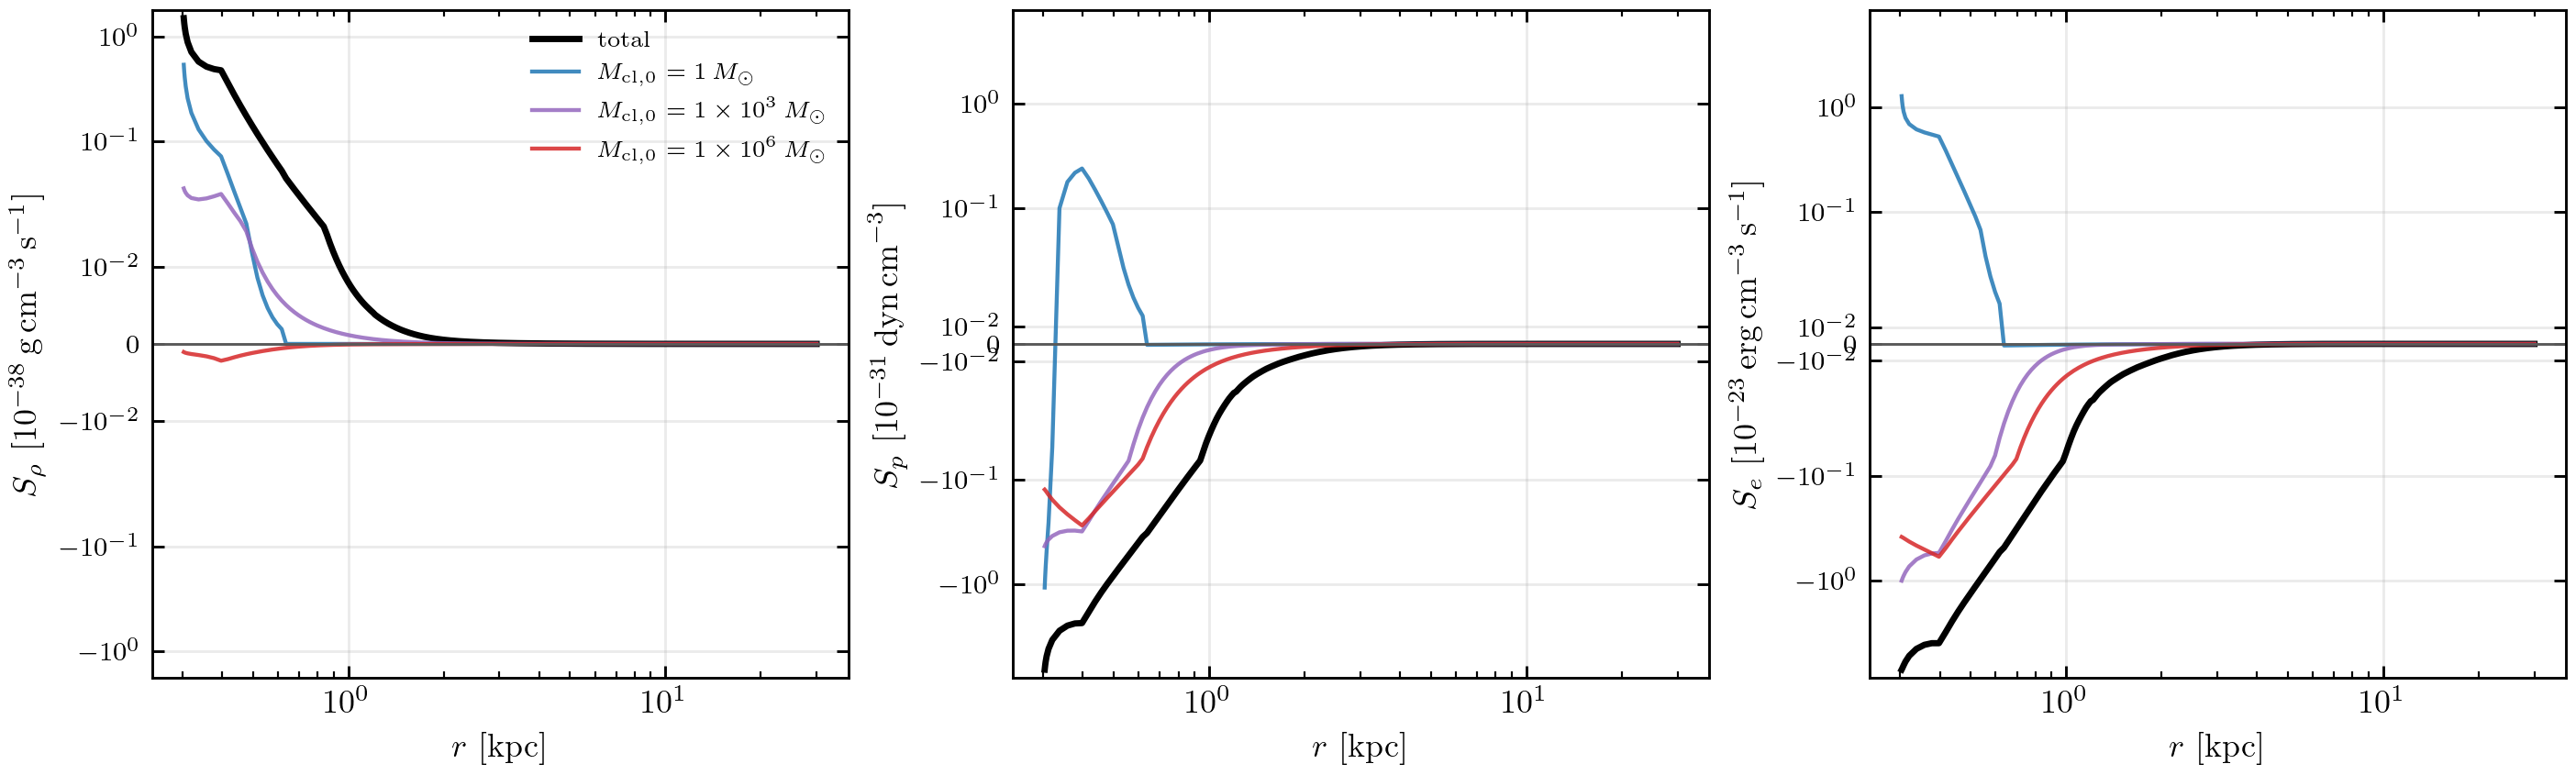
\includegraphics[width=\textwidth]{figures/cloud_coupling_source_terms.png}
\caption{
Signed cloud back-reaction source terms for the fiducial solved model.
The panels show the cloud contribution to the hot-phase mass, momentum, and energy source densities, following the sign conventions in Equations~(\ref{eq:hot_mass_source})--(\ref{eq:hot_energy_source}) but omitting the direct supernova source terms and hot radiative cooling term.
Each y-axis is scaled by the power of ten shown in its label.
Positive values add the corresponding conserved quantity to the hot phase, while negative values remove it.
The black curve is the sum over all cloud species; colored curves show representative low-, intermediate-, and high-mass species.
}
\label{fig:cloud_coupling_source_terms}
\end{figure*}

\subsection{Column-Density Velocity Profiles}
\label{subsec:model_observables}

The primary observable predicted by the model is the cool-gas column-density velocity distribution.
This is the step that connects the radial cloud trajectories to absorption-line data.
For cloud species $i$, the cold mass density along the flow is
\begin{equation}
\rho_{{\rm cold},i}
=
\frac{\dot{N}_i M_i}
{\Omega_{\rm wind}r^2v_i},
\end{equation}
and the corresponding hydrogen number density is
\begin{equation}
n_{{\rm H},i}
=
\frac{\rho_{{\rm cold},i}}{\mu_{\rm cool}m_p}.
\end{equation}
For monotonic cloud velocity histories,
\begin{equation}
\frac{dN}{dv}
\simeq
\sum_i
\frac{n_{{\rm H},i}}{\left|dv_i/dr\right|}.
\end{equation}
Only active cloud segments contribute to this transform.
If a species has been destroyed, it should not continue to add column at its final numerical velocity.
In practice, the observable calculation evaluates each species on the model radial grid, removes inactive segments, and interpolates the resulting contribution onto a common velocity grid before summing over species.
This species-resolved treatment is important because different initial cloud masses populate different velocity ranges.

For the binned observable used later in the paper, we instead compute a kernel-smoothed profile,
\begin{equation}
\left(\frac{dN}{dv}\right)_k
=
\sum_i
\int
n_{{\rm H},i}(r)
K_\sigma\left[v_i(r)-v_k\right]\,dr .
\end{equation}
Velocity moments and compact shape summaries are computed from this same profile.
The total column-density profile is therefore not determined by a single cloud acceleration history.
It is a weighted sum over survival, acceleration, and number density across the full cloud mass spectrum.
Figure~\ref{fig:cloud_species_dndv_contributions} shows this decomposition for the fiducial model.
The inference machinery introduced below operates on these predicted observable summaries rather than directly on the internal cloud trajectories.

\begin{figure}[!htbp]
\centering
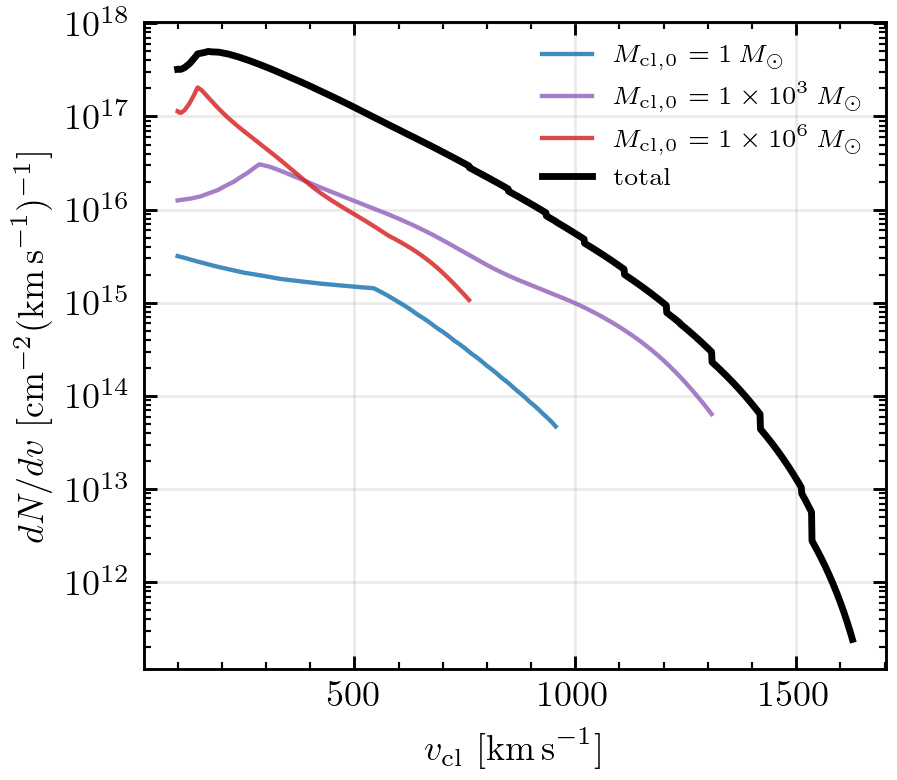
\includegraphics[width=\columnwidth]{figures/cloud_species_dndv_contributions.png}
\caption{
Species-resolved contribution to the cool-gas column-density velocity profile for the fiducial solved model.
The black curve is the total $dN/dv$ summed over all active cloud species.
The colored curves show representative low-, intermediate-, and high-mass species.
The low-mass species contributes at relatively low column because it is rapidly depleted, while the longer-lived species populate the higher-velocity part of the profile.
This decomposition is the observable counterpart of the mass and velocity histories in Figure~\ref{fig:cloud_species_mass_velocity_evolution}.
}
\label{fig:cloud_species_dndv_contributions}
\end{figure}
